\chapter{Kinematic Chain}

% Put the original image on the page
\begin{figure}[h]
    \centering
    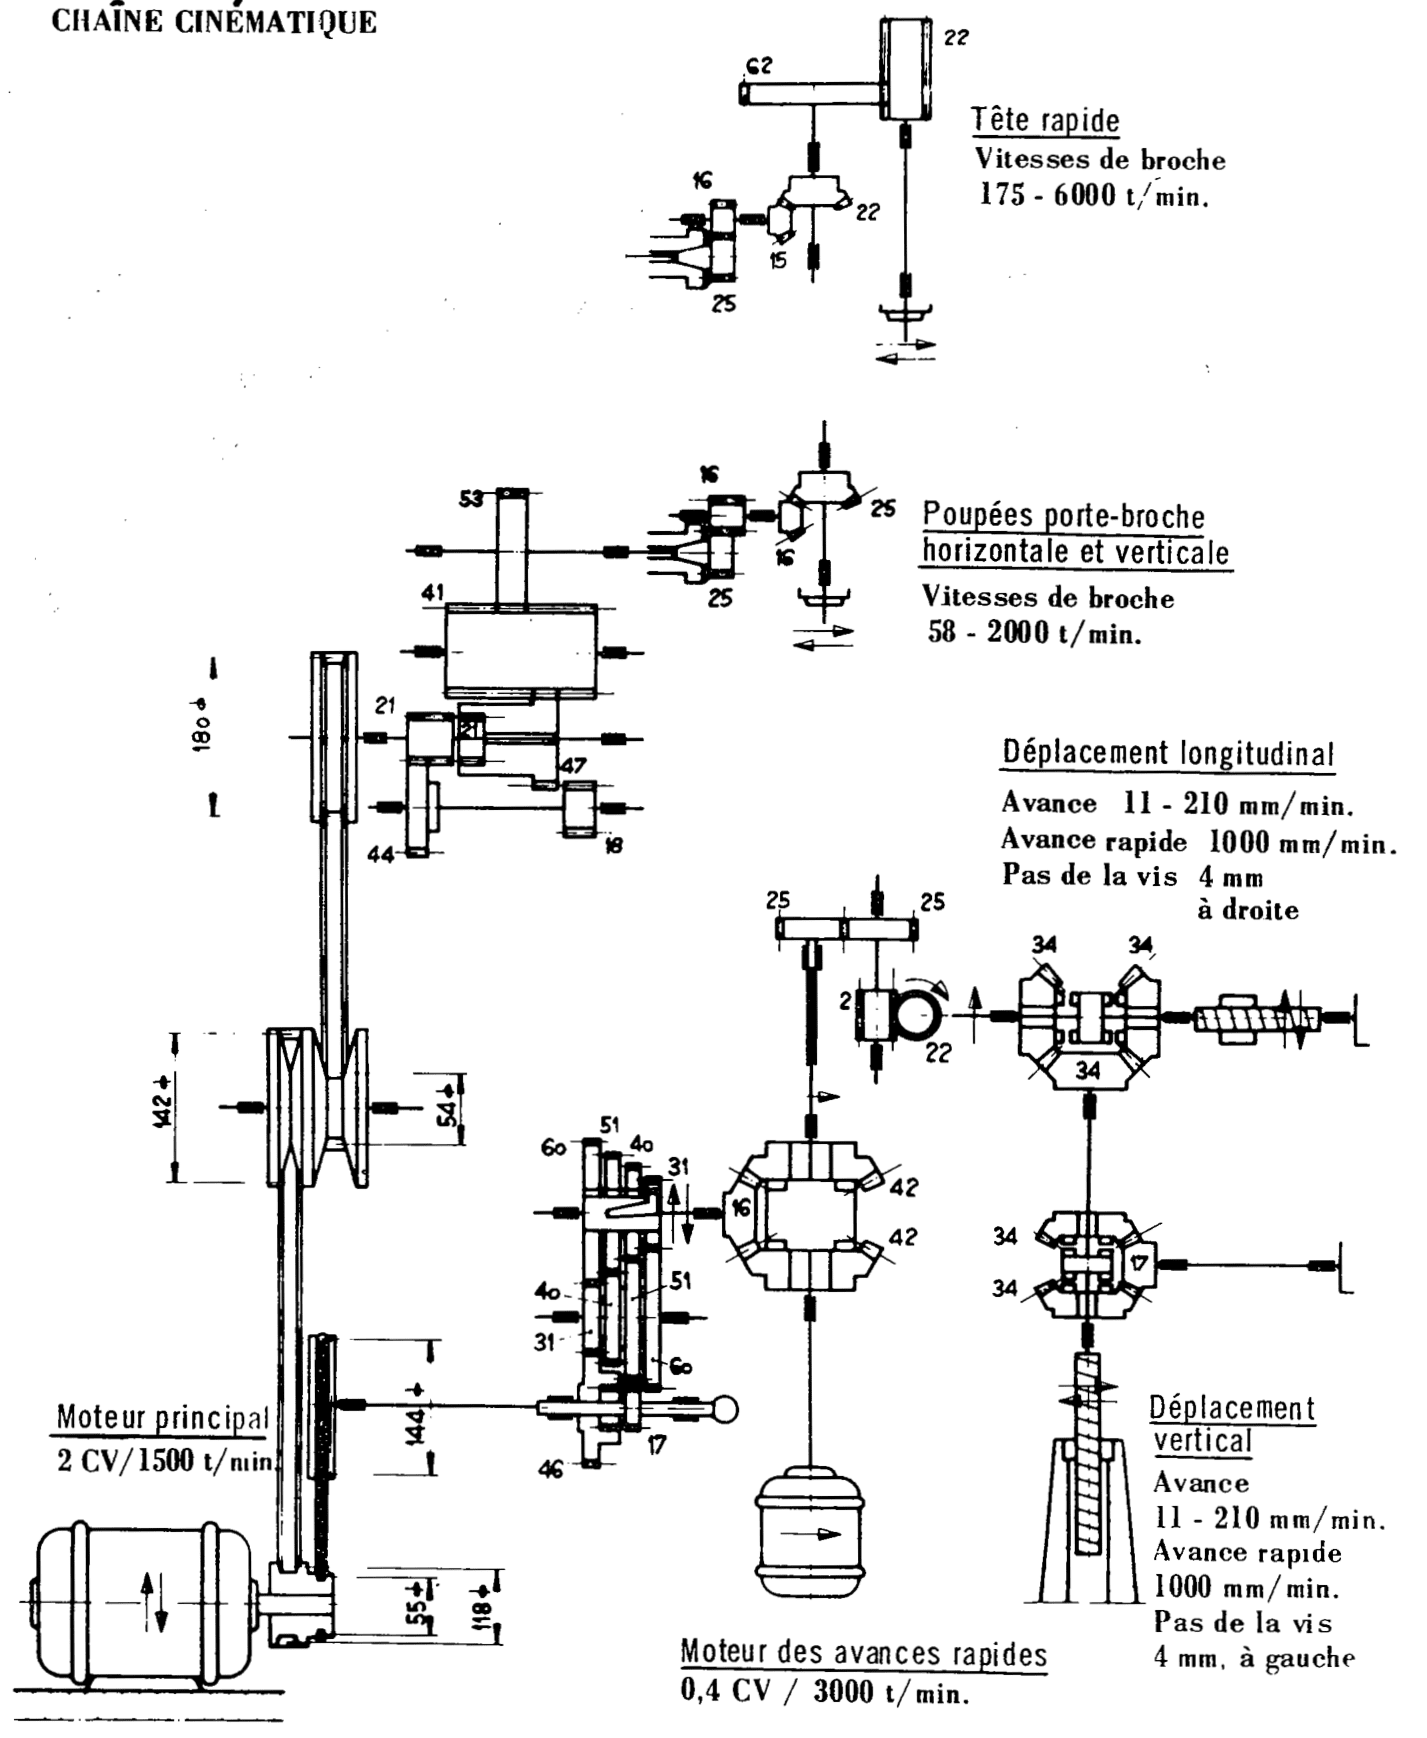
\includegraphics[width=0.95\linewidth]{images/page_56_in_13_36_kinematic_chain}
    \label{fig:kinematic_chain}
\end{figure}

% cover "Chaîne Cinématique with a white box.
\cover{80}{90}{4}{1}

% Default width for label blocks
\newlength{\labelBlockWidth}
\setlength{\labelBlockWidth}{5cm}

% Custom command for label block
\newcommand{\labelBlock}[4][\labelBlockWidth]{%
% Define a label block with white background, bold, and underlined text
    \begin{textblock*}{#1}(#2)
        \colorbox{white}{\parbox{\linewidth}{\uline{#3} \\ \small #4}\vspace{2pt}}
    \end{textblock*}%
}

% Cover "tête rapide" with an English version
\labelBlock{370pt,140pt}{\textbf{High Speed Head}}{Spindle Speeds \\
175 - 6000 r.p.m.}

% cover "Poupées porte-broche horizontale et verticale" with a white box since the new
% text doesn't cover it completely.
\cover{355}{252}{4}{2}
% Cover "Poupées porte-broche horizontale et verticale" with an English version
\labelBlock{355pt,252pt}{\textbf{Horizontal and} \\ \textbf{vertical spindles}}{Spindle Speeds \\
58 - 2000 r.p.m.}

% cover "Déplacement Longitudinal" with a white box since the new
% text doesn't cover it completely.
\cover{370}{330}{4}{2}
% Cover "Déplacement Longitudinal" with an English version
\labelBlock{370pt,335pt}{\textbf{Longitudinal movements}}{Feed: 11 - 210 mm/min \\
Rapid Feed: 1000 mm/min \\
4 mm right-hand thread}

% cover "Déplacement Vertical" with a white box since the new
% text doesn't cover it completely.
\cover{425}{520}{4}{5}

% Cover "Déplacement Vertical" with a white box
\labelBlock[5cm]{425pt,520pt}{\textbf{Vertical movements}}{Feed: 11 - 210 mm/min \\
Rapid Feed: 1000 mm/min \\
4 mm left-hand thread}

% Cover "Moteurs des avances rapides" with an English version
\labelBlock{280pt,600pt}{\textbf{Rapid Feed Motor}}{0.4 HP / 3000 r.p.m.}

% Cover "Moteur Principal" with an English version
\labelBlock[3.3cm]{65pt,535pt}{\textbf{Main Motor}}{2 HP / 1500 r.p.m.}
